% Options for packages loaded elsewhere
\PassOptionsToPackage{unicode}{hyperref}
\PassOptionsToPackage{hyphens}{url}
\PassOptionsToPackage{dvipsnames,svgnames,x11names}{xcolor}
%
\documentclass[
  12pt,
]{article}

\usepackage{amsmath,amssymb}
\usepackage{setspace}
\usepackage{iftex}
\ifPDFTeX
  \usepackage[T1]{fontenc}
  \usepackage[utf8]{inputenc}
  \usepackage{textcomp} % provide euro and other symbols
\else % if luatex or xetex
  \usepackage{unicode-math}
  \defaultfontfeatures{Scale=MatchLowercase}
  \defaultfontfeatures[\rmfamily]{Ligatures=TeX,Scale=1}
\fi
\usepackage{lmodern}
\ifPDFTeX\else  
    % xetex/luatex font selection
    \setmainfont[]{Times New Roman}
\fi
% Use upquote if available, for straight quotes in verbatim environments
\IfFileExists{upquote.sty}{\usepackage{upquote}}{}
\IfFileExists{microtype.sty}{% use microtype if available
  \usepackage[]{microtype}
  \UseMicrotypeSet[protrusion]{basicmath} % disable protrusion for tt fonts
}{}
\makeatletter
\@ifundefined{KOMAClassName}{% if non-KOMA class
  \IfFileExists{parskip.sty}{%
    \usepackage{parskip}
  }{% else
    \setlength{\parindent}{0pt}
    \setlength{\parskip}{6pt plus 2pt minus 1pt}}
}{% if KOMA class
  \KOMAoptions{parskip=half}}
\makeatother
\usepackage{xcolor}
\setlength{\emergencystretch}{3em} % prevent overfull lines
\setcounter{secnumdepth}{5}
% Make \paragraph and \subparagraph free-standing
\makeatletter
\ifx\paragraph\undefined\else
  \let\oldparagraph\paragraph
  \renewcommand{\paragraph}{
    \@ifstar
      \xxxParagraphStar
      \xxxParagraphNoStar
  }
  \newcommand{\xxxParagraphStar}[1]{\oldparagraph*{#1}\mbox{}}
  \newcommand{\xxxParagraphNoStar}[1]{\oldparagraph{#1}\mbox{}}
\fi
\ifx\subparagraph\undefined\else
  \let\oldsubparagraph\subparagraph
  \renewcommand{\subparagraph}{
    \@ifstar
      \xxxSubParagraphStar
      \xxxSubParagraphNoStar
  }
  \newcommand{\xxxSubParagraphStar}[1]{\oldsubparagraph*{#1}\mbox{}}
  \newcommand{\xxxSubParagraphNoStar}[1]{\oldsubparagraph{#1}\mbox{}}
\fi
\makeatother


\providecommand{\tightlist}{%
  \setlength{\itemsep}{0pt}\setlength{\parskip}{0pt}}\usepackage{longtable,booktabs,array}
\usepackage{calc} % for calculating minipage widths
% Correct order of tables after \paragraph or \subparagraph
\usepackage{etoolbox}
\makeatletter
\patchcmd\longtable{\par}{\if@noskipsec\mbox{}\fi\par}{}{}
\makeatother
% Allow footnotes in longtable head/foot
\IfFileExists{footnotehyper.sty}{\usepackage{footnotehyper}}{\usepackage{footnote}}
\makesavenoteenv{longtable}
\usepackage{graphicx}
\makeatletter
\newsavebox\pandoc@box
\newcommand*\pandocbounded[1]{% scales image to fit in text height/width
  \sbox\pandoc@box{#1}%
  \Gscale@div\@tempa{\textheight}{\dimexpr\ht\pandoc@box+\dp\pandoc@box\relax}%
  \Gscale@div\@tempb{\linewidth}{\wd\pandoc@box}%
  \ifdim\@tempb\p@<\@tempa\p@\let\@tempa\@tempb\fi% select the smaller of both
  \ifdim\@tempa\p@<\p@\scalebox{\@tempa}{\usebox\pandoc@box}%
  \else\usebox{\pandoc@box}%
  \fi%
}
% Set default figure placement to htbp
\def\fps@figure{htbp}
\makeatother
% definitions for citeproc citations
\NewDocumentCommand\citeproctext{}{}
\NewDocumentCommand\citeproc{mm}{%
  \begingroup\def\citeproctext{#2}\cite{#1}\endgroup}
\makeatletter
 % allow citations to break across lines
 \let\@cite@ofmt\@firstofone
 % avoid brackets around text for \cite:
 \def\@biblabel#1{}
 \def\@cite#1#2{{#1\if@tempswa , #2\fi}}
\makeatother
\newlength{\cslhangindent}
\setlength{\cslhangindent}{1.5em}
\newlength{\csllabelwidth}
\setlength{\csllabelwidth}{3em}
\newenvironment{CSLReferences}[2] % #1 hanging-indent, #2 entry-spacing
 {\begin{list}{}{%
  \setlength{\itemindent}{0pt}
  \setlength{\leftmargin}{0pt}
  \setlength{\parsep}{0pt}
  % turn on hanging indent if param 1 is 1
  \ifodd #1
   \setlength{\leftmargin}{\cslhangindent}
   \setlength{\itemindent}{-1\cslhangindent}
  \fi
  % set entry spacing
  \setlength{\itemsep}{#2\baselineskip}}}
 {\end{list}}
\usepackage{calc}
\newcommand{\CSLBlock}[1]{\hfill\break\parbox[t]{\linewidth}{\strut\ignorespaces#1\strut}}
\newcommand{\CSLLeftMargin}[1]{\parbox[t]{\csllabelwidth}{\strut#1\strut}}
\newcommand{\CSLRightInline}[1]{\parbox[t]{\linewidth - \csllabelwidth}{\strut#1\strut}}
\newcommand{\CSLIndent}[1]{\hspace{\cslhangindent}#1}

\makeatletter
\@ifpackageloaded{caption}{}{\usepackage{caption}}
\AtBeginDocument{%
\ifdefined\contentsname
  \renewcommand*\contentsname{Table of contents}
\else
  \newcommand\contentsname{Table of contents}
\fi
\ifdefined\listfigurename
  \renewcommand*\listfigurename{List of Figures}
\else
  \newcommand\listfigurename{List of Figures}
\fi
\ifdefined\listtablename
  \renewcommand*\listtablename{List of Tables}
\else
  \newcommand\listtablename{List of Tables}
\fi
\ifdefined\figurename
  \renewcommand*\figurename{Figure}
\else
  \newcommand\figurename{Figure}
\fi
\ifdefined\tablename
  \renewcommand*\tablename{Table}
\else
  \newcommand\tablename{Table}
\fi
}
\@ifpackageloaded{float}{}{\usepackage{float}}
\floatstyle{ruled}
\@ifundefined{c@chapter}{\newfloat{codelisting}{h}{lop}}{\newfloat{codelisting}{h}{lop}[chapter]}
\floatname{codelisting}{Listing}
\newcommand*\listoflistings{\listof{codelisting}{List of Listings}}
\makeatother
\makeatletter
\makeatother
\makeatletter
\@ifpackageloaded{caption}{}{\usepackage{caption}}
\@ifpackageloaded{subcaption}{}{\usepackage{subcaption}}
\makeatother

\usepackage{bookmark}

\IfFileExists{xurl.sty}{\usepackage{xurl}}{} % add URL line breaks if available
\urlstyle{same} % disable monospaced font for URLs
\hypersetup{
  pdftitle={From Data to Action: Leveraging Bike-Sharing Patterns},
  pdfauthor={Izzul Fattah Aji Pratama; Thuy Nhu Nguyen; Bhuvana Chandrasekar},
  colorlinks=true,
  linkcolor={blue},
  filecolor={Maroon},
  citecolor={Blue},
  urlcolor={Blue},
  pdfcreator={LaTeX via pandoc}}


\title{\textbf{From Data to Action: Leveraging Bike-Sharing Patterns}}
\author{Izzul Fattah Aji Pratama \and Thuy Nhu Nguyen \and Bhuvana
Chandrasekar}
\date{2025-05-26}

\begin{document}
\maketitle

\renewcommand*\contentsname{Table of contents}
{
\hypersetup{linkcolor=}
\setcounter{tocdepth}{2}
\tableofcontents
}

\setstretch{1.5}
\section{Executive Summary}\label{executive-summary}

This report analyzes two years of data from Washington D.C.'s Capital
Bikeshare system, revealing how environmental and temporal factors
influence bike usage patterns. The findings highlight the strong link
between favorable weather, holidays, and bike rental trends, with
implications for urban transport systems.

Applying these insights to Australia, the report underscores the
significant role of cycling culture, particularly among university
students, in sustaining bike-sharing programs like Lime e-bikes. The
study emphasizes the potential of bike-sharing systems to promote
sustainable, healthy, and efficient mobility.

\section{Introduction}\label{introduction}

Urban transportation is shifting toward more sustainable and efficient
mobility solutions. Bike-sharing programs have emerged as a popular
option, offering flexible access to bicycles, including e-bikes for
short-distance urban travel. These systems help reduce traffic
congestion, lower emissions, and promote healthy lifestyles.

This report analyzes two years of data from the Capital Bikeshare system
in Washington D.C. (2011--2012), capturing rental patterns across time
and weather conditions. The dataset includes both daily and hourly
records with variables such as temperature, humidity, season, weekday,
and user type.

We explore how environmental and temporal factors affect rental demand,
user composition, and daily usage trends. Although U.S.-based, the
findings are highly applicable to Australian cities, where cycling is a
practical and cultural norm, especially among university students.

Campuses often encourage cycling by design, creating ideal conditions
for bike-sharing success. Insights from this study can support better
planning, resource allocation, and policy development for shared
mobility services in Australian urban settings.

\begin{center}\rule{0.5\linewidth}{0.5pt}\end{center}

\section{Summary of Insights}\label{summary-of-insights}

\begin{longtable}[]{@{}ll@{}}
\toprule\noalign{}
Feature & Effect on Rentals \\
\midrule\noalign{}
\endhead
\bottomrule\noalign{}
\endlastfoot
Temperature & Strong positive impact \\
Feels-like Temp & Similar to temperature \\
Humidity & Mild negative impact \\
Windspeed & Weak correlation \\
Hour of Day & Peaks during morning and evening commute \\
Weekday vs Weekend & Higher and consistent on weekdays \\
Time Progression & General upward trend year over year \\
\end{longtable}

\begin{center}\rule{0.5\linewidth}{0.5pt}\end{center}

\section{Methodology:}\label{methodology}

This report uses the Bike Sharing Dataset from Washington D.C., which
contains hourly and daily records for 2011--2012 (Fanaee-T \& Gama,
2014).It contains two files: \texttt{day.csv}(daily rental data) and
\texttt{hour.csv} (hourly rental data) from 2011 to 2012 in Washington
D.C.

The datasets are complete, with no missing values. They contain weather
metrics, timestamps, and detailed user counts. We categorized the
variables into three analytical areas:

1. \textbf{Environmental conditions}: Continuous variables include
temperature (\texttt{temp}), perceived temperature (\texttt{atemp}),
humidity (\texttt{hum}), and windspeed (\texttt{windspeed}) --- all
normalized. These were sourced from `hour.csv` and used to assess how
weather influences demand.

2. \textbf{Temporal factors}: These include hour of day (\texttt{hr}),
day of week (\texttt{weekday}), holidays, and working days
(\texttt{workingday}). \texttt{hour.csv}was used to examine hourly
rental patterns and compare weekdays to weekends. Seasonal trends were
analyzed using \texttt{season} (1 = Winter, 2 = Spring, 3 = Summer, 4 =
Fall) and \texttt{mnth} from \texttt{day.csv}.

3. \textbf{User behavior}: Total rentals (\texttt{cnt}) are split into
\texttt{casual}(non-registered) and \texttt{registered} (subscribers).
\texttt{day.csv} was used to study seasonal variation in user types,
while \texttt{hour.csv} was used for finer temporal granularity.

All analysis was performed in \textbf{R}, using \texttt{tidyverse} for
data wrangling and \texttt{ggplot2} for visualization. The report was
built in \textbf{Quarto} for reproducibility, and \textbf{Git} was used
for structured collaboration via separate branches.

Figure~\ref{fig-season-users} shows average total users by season using
\texttt{day.csv}, capturing clear seasonal demand shifts.

Table~\ref{tbl-hourly-weektype} uses \texttt{hour.csv} to show average
hourly rentals on weekdays vs.~weekends, demonstrating time-of-day
behavioral differences. Further analysis appears in the Results section.

\begin{figure}

\centering{

\pandocbounded{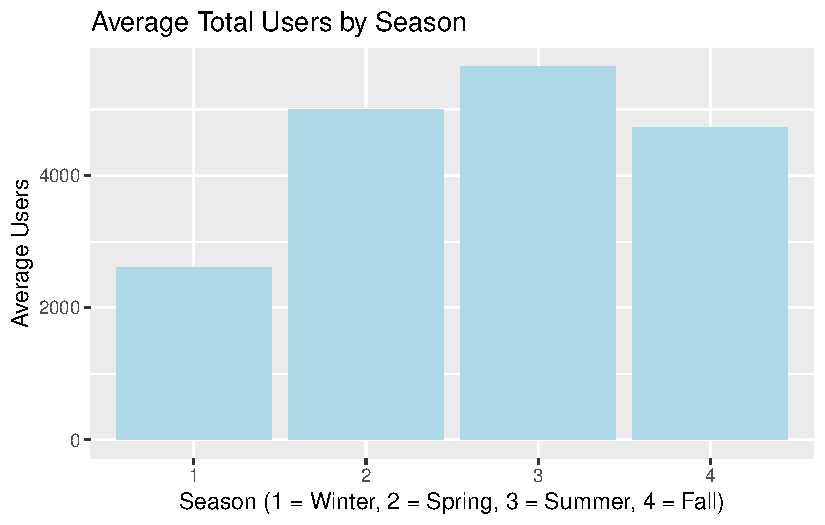
\includegraphics[keepaspectratio]{group-work--assignment-3_files/figure-pdf/fig-season-users-1.pdf}}

}

\caption{\label{fig-season-users}Average Total Users by Season}

\end{figure}%

\begin{longtable}[]{@{}rrr@{}}

\caption{\label{tbl-hourly-weektype}Average Hourly Rentals on Weekdays
vs Weekends}

\tabularnewline

\toprule\noalign{}
hr & Weekday & Weekend \\
\midrule\noalign{}
\endhead
\bottomrule\noalign{}
\endlastfoot
0 & 37.6 & 94.1 \\
1 & 17.5 & 72.6 \\
2 & 9.4 & 56.0 \\
3 & 5.2 & 27.0 \\
4 & 5.4 & 8.5 \\
5 & 24.3 & 8.5 \\
6 & 99.5 & 17.8 \\
7 & 282.1 & 39.5 \\
8 & 464.6 & 99.2 \\
9 & 238.7 & 171.7 \\
10 & 138.1 & 261.2 \\
11 & 161.9 & 322.0 \\
12 & 204.3 & 374.2 \\
13 & 202.5 & 380.2 \\
14 & 187.7 & 372.5 \\
15 & 203.9 & 368.2 \\
16 & 292.3 & 360.8 \\
17 & 515.9 & 326.6 \\
18 & 483.2 & 282.3 \\
19 & 343.3 & 232.7 \\
20 & 246.8 & 174.4 \\
21 & 184.6 & 141.8 \\
22 & 137.2 & 116.8 \\
23 & 87.5 & 88.7 \\

\end{longtable}

\section{Results:}\label{results}

\subsection{Hourly and Weather-Based Rental
Patterns}\label{hourly-and-weather-based-rental-patterns}

As shown in Figure~\ref{fig-hourly-rentals}, rental activity varies by
time of day and day type. On weekdays, \textbf{registered users} drive
sharp peaks around \textbf{8 AM and 5--6 PM}, aligning with typical
commute hours. On weekends, rentals are more evenly distributed, with
\textbf{casual users} becoming more prominent around midday. This
pattern reveals distinct behavioral trends between commuter and leisure
riders. Figure~\ref{fig-weather-scatter} shows that \textbf{temperature}
and \textbf{apparent temperature} positively correlate with total
rentals, while \textbf{humidity} and \textbf{windspeed} have weaker
negative effects (Li et al., 2015). These findings highlight the
combined impact of structured routines and weather conditions on
bike-sharing demand.

\subsection{Seasonal Trends and User
Behavior}\label{seasonal-trends-and-user-behavior}

To examine how bike usage shifts across seasons, we analyzed total
rentals (\texttt{cnt}) and user type composition.
Figure~\ref{fig-user-by-season} hows that demand peaks in summer and
fall, while winter records the lowest activity.
Table~\ref{tbl-user-share-by-season} breaks down usage by user type,
revealing that registered users dominate in all seasons but especially
in winter, suggesting habitual commuting behavior. In contrast, casual
user activity more than doubles in summer, indicating recreational or
tourist usage. These seasonal shifts suggest that demand is driven by
both weather and user intent, with commuters being more consistent and
casual users more season-sensitive.

\begin{figure}

\centering{

\pandocbounded{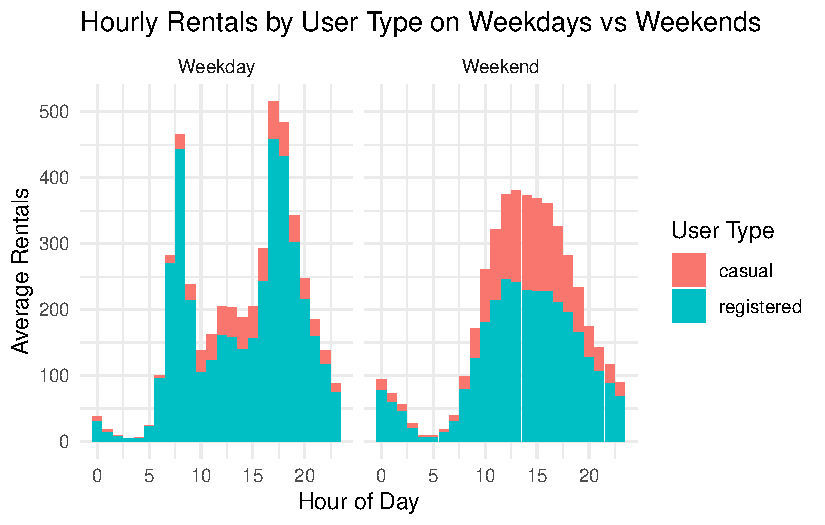
\includegraphics[keepaspectratio]{group-work--assignment-3_files/figure-pdf/fig-hourly-rentals-1.pdf}}

}

\caption{\label{fig-hourly-rentals}Average Hourly Bike Rentals on
Weekdays vs Weekends}

\end{figure}%

\begin{figure}

\centering{

\pandocbounded{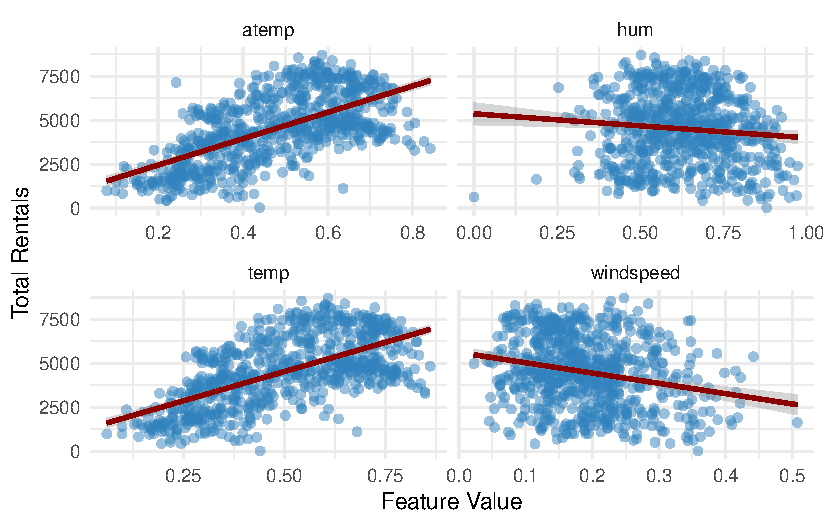
\includegraphics[keepaspectratio]{group-work--assignment-3_files/figure-pdf/fig-weather-scatter-1.pdf}}

}

\caption{\label{fig-weather-scatter}Weather Features vs.~Total Bike
Rentals}

\end{figure}%

\begin{figure}

\centering{

\pandocbounded{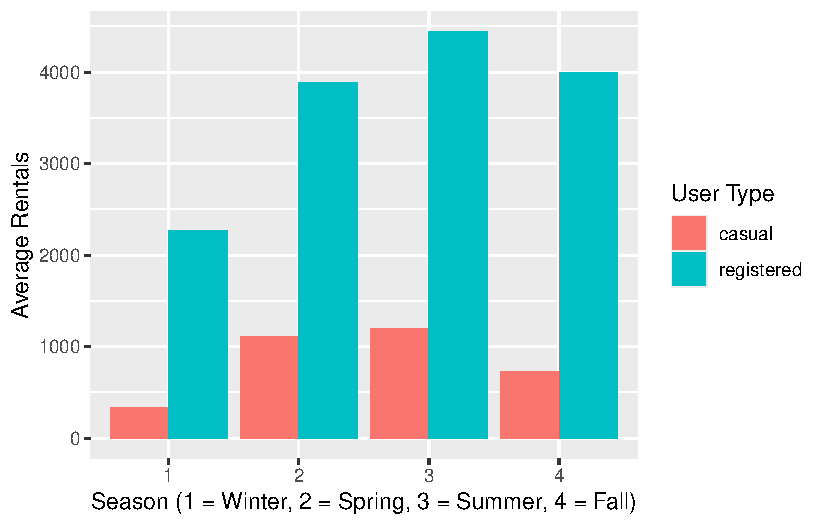
\includegraphics[keepaspectratio]{group-work--assignment-3_files/figure-pdf/fig-user-by-season-1.pdf}}

}

\caption{\label{fig-user-by-season}Average Casual and Registered Users
by Season}

\end{figure}%

\begin{longtable}[]{@{}rrr@{}}

\caption{\label{tbl-user-share-by-season}Percentage of Casual and
Registered Users by Season}

\tabularnewline

\toprule\noalign{}
season & pct\_casual & pct\_registered \\
\midrule\noalign{}
\endhead
\bottomrule\noalign{}
\endlastfoot
1 & 12.9 & 87.1 \\
2 & 22.2 & 77.8 \\
3 & 21.3 & 78.7 \\
4 & 15.4 & 84.6 \\

\end{longtable}

\section{Discussion, Conclusion and
Recommendations:}\label{discussion-conclusion-and-recommendations}

This report set out to explore how environmental and temporal factors
influence bike rental demand in Washington D.C., using the UCI Bike
Sharing Dataset. We investigated rental patterns by season, weather
conditions, temperature, hour of day, and user type (casual
vs.~registered), with the goal of uncovering meaningful trends to inform
data-driven decision-making.

Our findings revealed strong seasonal and hourly patterns. Rental demand
peaked in summer and fall, with a surge in casual user activity during
warmer months --- suggesting weather-sensitive, potentially
tourist-driven behavior. In contrast, registered users displayed
consistent usage throughout the year and weekdays, indicative of
habitual commuting. Rental volumes also followed predictable daily
cycles, with distinct peaks during morning and evening commute hours and
more gradual midday rises on weekends.

These trends show that registered users form a reliable commuter base,
while casual users introduce seasonal and environmental variability.
This distinction is critical for bike-sharing companies, city planners,
and transportation authorities when developing policies, allocating
fleet resources, and adjusting marketing strategies.

We recommend:

\begin{itemize}
\tightlist
\item
  Increasing bike availability and docking stations near recreational or
  high-footfall areas in summer
\item
  Ensuring year-round service quality and infrastructure for
  commuter-heavy routes
\item
  Using time-based demand trends to optimize staff scheduling,
  re-balancing logistics, and promotional campaigns
\end{itemize}

Importantly, our analysis is reproducible and adaptable. The approach we
used --- integrating open data with R, Quarto, and Git --- can be
applied to other cities, climates, or shared mobility services. Whether
for city governments, local councils, or private operators managing
bikes or e-scooters, these insights can help refine network planning,
predict usage peaks, position vehicles more effectively, and even plan
battery charging or maintenance station locations in electric fleets.

\section{AI Acknowledgment}\label{ai-acknowledgment}

There are AI support for grammar checking, using OpenAI.
\href{https://chatgpt.com/share/683412ac-5054-8002-8523-a5a1b400ef0a}{Link}

\section*{References}\label{references}
\addcontentsline{toc}{section}{References}

\phantomsection\label{refs}
\begin{CSLReferences}{1}{0}
\bibitem[\citeproctext]{ref-fanaee2014event}
Fanaee-T, H., \& Gama, J. (2014). \emph{Event labeling combining
ensemble detectors and background knowledge}.
\url{https://archive.ics.uci.edu/ml/datasets/Bike+Sharing+Dataset}.

\bibitem[\citeproctext]{ref-li2015bike}
Li, W., Zhang, Y., \& Chen, C. (2015). Bike sharing and weather: Impact
analysis and operational strategies. \emph{Transportation Research Part
C: Emerging Technologies}, \emph{86}, 95--108.

\end{CSLReferences}




\end{document}
